\begin{frame}[t, fragile]{Customização}
  \begin{itemize}
    \item Existem muitas opções
    \begin{itemize}
      \item Diferentes tipos de gráficos
      \item Diversas customizações
    \end{itemize}
    \item A escolha depende
    \begin{itemize}
      \item Dados
      \item Estória a ser contada
    \end{itemize}
  \end{itemize}
\end{frame}
%
\begin{frame}[t, fragile]{Customização}
  \begin{columns}
    \begin{column}{0.55\textwidth}
        \lstinputlisting[language=python]{aula-2/codigos/matplotlib/matplotlib-customization-1.py}  
    \end{column}

    \begin{column}{0.45\textwidth}
      \begin{center}
        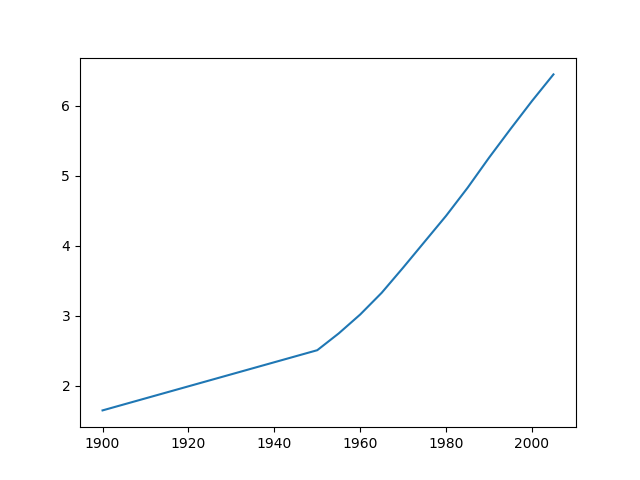
\includegraphics[scale=.35]{aula-2/figuras/matplotlib-customization-1.png}
      \end{center}
    \end{column}
  \end{columns}
\end{frame}
%
\begin{frame}[t, fragile]{Títulos dos eixos X e Y}
  \begin{columns}
    \begin{column}{0.55\textwidth}
        \lstinputlisting[language=python]{aula-2/codigos/matplotlib/matplotlib-customization-2.py}  
    \end{column}

    \begin{column}{0.45\textwidth}
      \begin{center}
        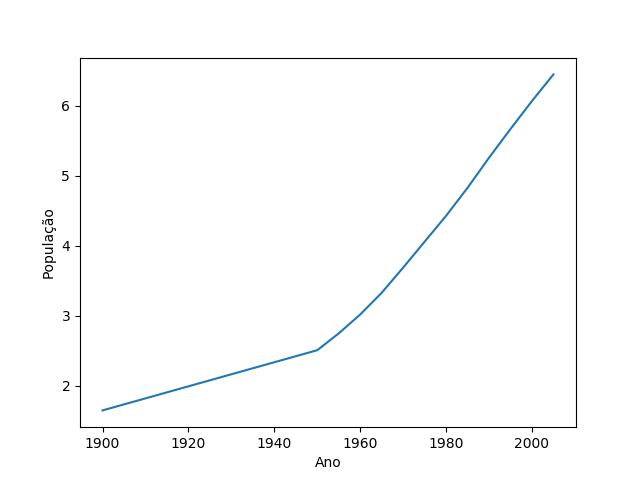
\includegraphics[scale=.35]{aula-2/figuras/matplotlib-customization-2.png}
      \end{center}
    \end{column}
  \end{columns}
\end{frame}
%
\begin{frame}[t, fragile]{Título Principal}
  \begin{columns}
    \begin{column}{0.55\textwidth}
        \lstinputlisting[language=python, firstline=12]{aula-2/codigos/matplotlib/matplotlib-customization-3.py}  
    \end{column}

    \begin{column}{0.45\textwidth}
      \begin{center}
        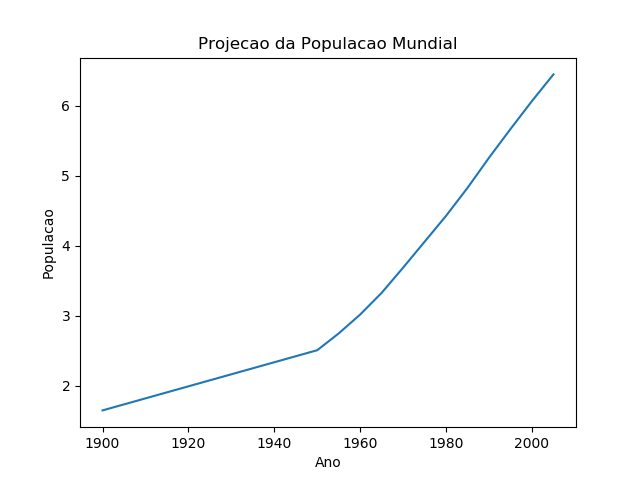
\includegraphics[scale=.35]{aula-2/figuras/matplotlib-customization-3.png}
      \end{center}
    \end{column}
  \end{columns}
\end{frame}
%
\begin{frame}[t, fragile, allowframebreaks]{Ticks}
  \begin{columns}
    \begin{column}{0.55\textwidth}
        \lstinputlisting[language=python, firstline=12]{aula-2/codigos/matplotlib/matplotlib-customization-4.py}  
    \end{column}

    \begin{column}{0.45\textwidth}
      \begin{center}
        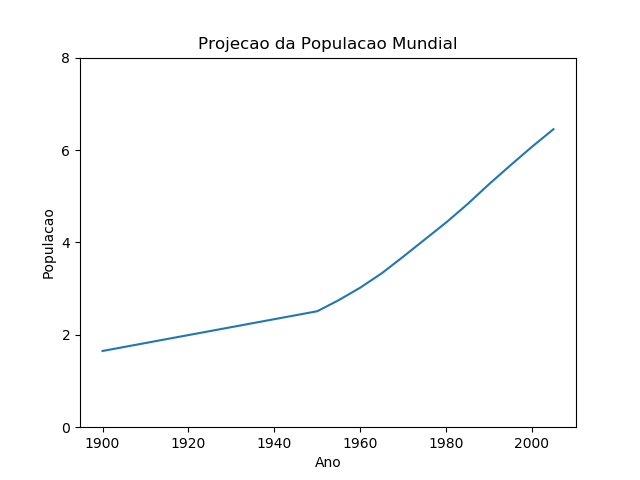
\includegraphics[scale=.35]{aula-2/figuras/matplotlib-customization-4.png}
      \end{center}
    \end{column}
  \end{columns}
  
  \framebreak
  
  \begin{columns}
    \begin{column}{0.55\textwidth}
        \lstinputlisting[language=python, firstline=12]{aula-2/codigos/matplotlib/matplotlib-customization-5.py}  
    \end{column}

    \begin{column}{0.45\textwidth}
      \begin{center}
        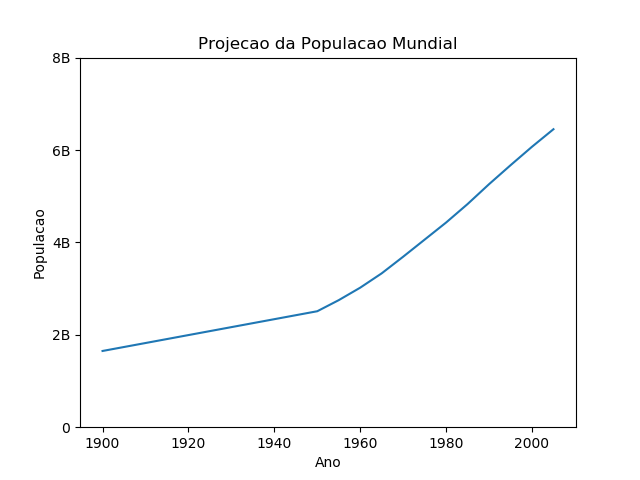
\includegraphics[scale=.35]{aula-2/figuras/matplotlib-customization-5.png}
      \end{center}
    \end{column}
  \end{columns}
\end{frame}
%
\begin{frame}[t, fragile]{Adicionando Dados Históricos}
  \begin{columns}
    \begin{column}{0.55\textwidth}
        \lstinputlisting[language=python, firstline=12]{aula-2/codigos/matplotlib/matplotlib-customization-6.py}  
    \end{column}

    \begin{column}{0.45\textwidth}
      \begin{center}
        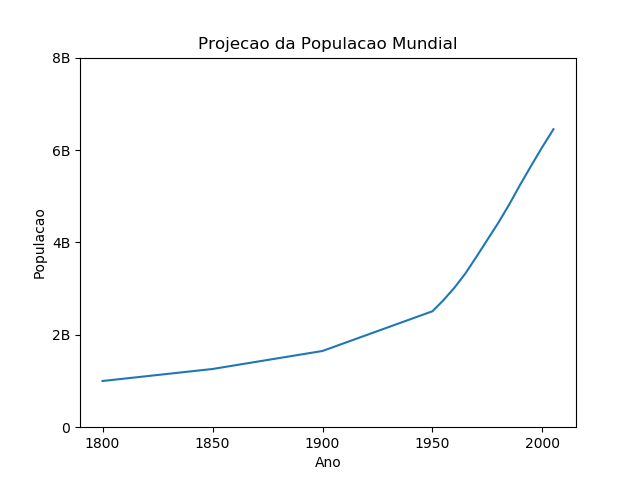
\includegraphics[scale=.35]{aula-2/figuras/matplotlib-customization-6.png}
      \end{center}
    \end{column}
  \end{columns} 
\end{frame}
%
%
\begin{frame}[t, fragile]{Antes x Depois}
  \begin{columns}
    \begin{column}{0.5\textwidth}
      \begin{figure}
        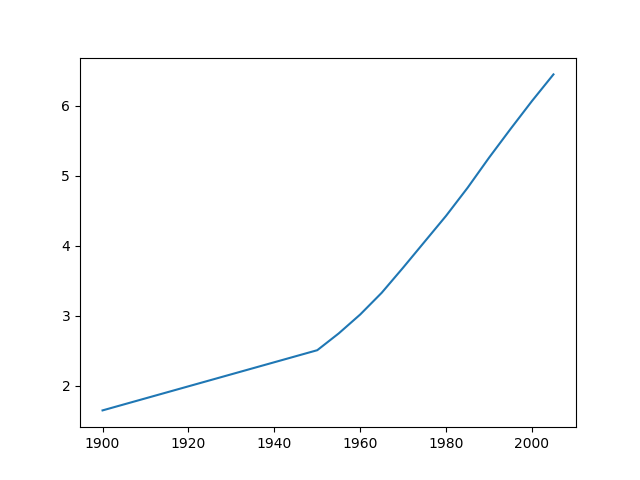
\includegraphics[scale=.35]{aula-2/figuras/matplotlib-customization-1.png}
      \end{figure}
    \end{column}

    \begin{column}{0.5\textwidth}
      \begin{figure}
        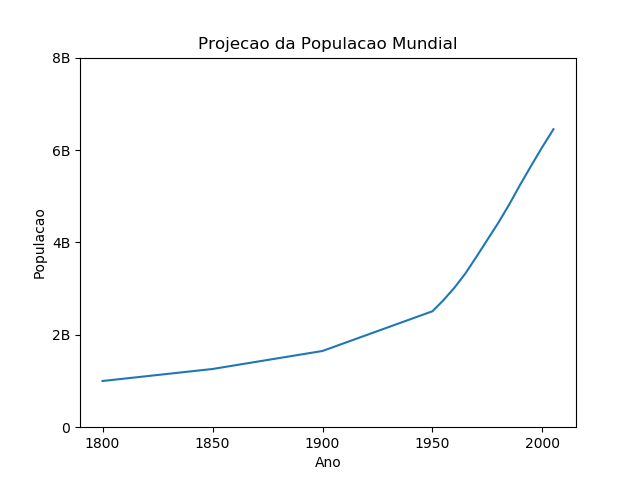
\includegraphics[scale=.35]{aula-2/figuras/matplotlib-customization-6.png}
      \end{figure}
    \end{column}
  \end{columns} 
\end{frame}

